\chapter{Monitoring DLAKaApp}
\todo{Better title. Is this one okay?}
% % This is the third result chapter which presents the first solution of the thesis.
% % The solution is integrated into the overall concept introduced in Chapter 4 and
% % it is technically based on the foundation described in Chapter 5.
% % A thesis should provide at least two such solutions.

\todo{Introduction to chapter}

\todo{Motivation}
The development of SPMonitor will be based on the following motivation story.
This extends the story of the BestRentalPoC.

The DrivingLicenseAuthorityKarlsruhe (DLAKa) wants to provide citizens with digital driving licenses,
which can, for example, be used to prove to a car rental company that they possess a valid driving license.
They hire the company ServiceProvider (SP) to develop and operate the system necessary for issuing and verifying
digital driving licenses. The contract specifies an initial payment for the development of the system
and afterward a yearly fee for the operation of the system.
After receiving the contract from DLAKa, SP starts designing the system
for DLAKa. Because SP has to operate the system on a fixed yearly budget,
they want to monitor the performance of the system to identify parts with excessive resource usage, which
incur additional costs. They identify the memory usage of the system as a technical metric that should be monitored.
This metric will be called MemUse (Memory Usage).
Additionally, \Gls{DLAKa} has asked SP to provide the capability of monitoring business metrics for them.
\Gls{DLAKa} wants to know how many digital driving licenses are being issued. 
This metric will be called NumDDL (Number of Issued Digital Driving Licenses).
To monitor both technical and business metrics, SP designs the ServiceProviderMonitor (SPMonitor) as a part
of the system for \Gls{DLAKa} which will provide all functionality for monitoring the specified metrics.

\section{Analysis}

The following section will provide an analysis of SPMonitor based on the motivation above.
Firstly, use cases are derived from the motivation above. These use cases are then used
to derive capabilities and requirements for SPMonitor. This will be followed by defining
the metrics that SPMonitor will collect. Finally, SPMonitor will be analyzed regarding its
integration with DLAKaApp and modifications which might have to be made in DLAKaApp.

\subsection{Use Cases}

\begin{figure}
	\centering
	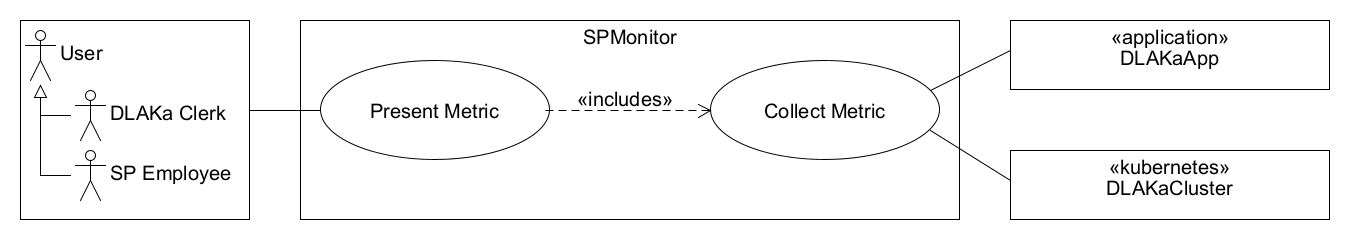
\includegraphics[width=\textwidth]{figures/2.1_use_case_spmonitor.png}
	\caption{Use Case Diagram: SPMonitor}
	\label{fig:use_case_diagram_spmonitor}
\end{figure}

% Based on the motivation, two use cases for SPMonitor were derived: Present Metric and Collect Metric.
% The use case Present Metric is concerned with the presentation of monitoring data to the users of SPMonitor.
% The use case Collect Metric meanwhile, focuses on the interaction between SPMonitor and the monitored system by describing
% how metrics should be collected. The relation of both use cases can be seen in Figure \ref{fig:use_case_diagram_spmonitor}.

% The use case Present Metric has only one primary actor who is a user.
% A user of SPMonitor can have one of two roles. Firstly, a user could work for DLAKa and thus have the role
% DLAKa Clerk. The other possibility is that the user could work for SP and have the role SP Employee.
% Due to possible privacy concerns, each user can only have one of these two roles.
% Based on their role they will be able to access different dashboards which contain different data.
% The only precondition of the use case is that the metric which the user wants to access is configured.
% Configuration of a metric means setting up the generation of the data in the monitored system as well
% as the collection and storage of the data by SPMonitor. This will be done as part of the development of SPMonitor.
% When the user opens the SPMonitor user interface, they will be able to view different dashboards.
% A dashboard presents related monitoring data as a collection of graphs.
% After selecting a dashboard, SPMonitor will retrieve the stored values for the dashboard and display
% them in graphs.
% Just like the configuration of the metrics, both the dashboards and the graphs will be created during
% the development of SPMonitor. This means that a user will not be able to change them.
% The full description of the Present Metric use case can be seen in Listing \ref{lis:use_case_description_present_metric}.

% \begin{lstlisting}[caption = {Use Case Description: Present Metric}, label = {lis:use_case_description_present_metric}, style = kit-cm, language=]
% Title: Present Metric

% Primary Actors: User

% Preconditions:
% - SPMonitor has the metric configured

% Flow:
% 1. User opens a dashboard for a metric
% 2. SPMonitor retrieves all stored values for that metric
% 3. SPMonitor displays the values in a graph

% Alternative Flows:
% 2a. SPMonitor has no values stored for the metric
% 2a1. SPMonitor displays a message that the metric has no stored values

% Information Requirements:
% - Values for the metric
% \end{lstlisting}

% The use case Collect Metric has no primary actors as it describes
% the interaction between the DLAKaApp and SPMonitor.
% This use case has three preconditions. The first is that the DLAKaApp is running
% inside a Kubernetes cluster called DLAKaCluster. Additionally, the DLAKaApp
% and the DLAKaCluster have to be set up to collect the NumDDL and MemUse metric respectively.
% As was explained for the Present Metric use case, this will be done during the development
% of SPMonitor.
% The flow for both metrics is the same except that SPMonitor interacts with the DLAKaApp for
% the NumDDL metric and with DLAKaCluster for the MemUse metric. To avoid duplication the flow
% will only be described once and the DLAKaApp and the DLAKaCluster will be
% referred to as the monitored system.
% First SPMonitor sends a request to the monitored system for the current value of its metric.
% The monitored system sends a reply with the current value. SPMonitor then receives the reply
% and stores the current value so that it can be accessed later. When SPMonitor stores a metric's
% value it will also keep previously stored values so that the latest value can be compared
% to historical data. Should the monitored system reply with an error message instead of a value for the requested metric,
% SPMonitor will restart the flow and retry to collect a current value for the metric.
% This flow results in the postcondition that SPMonitor has new values
% stored for both the NumDDL and MemUse metric.
% The full description of the Collect Metric use case can be seen in Listing \ref{lis:use_case_description_collect_metric}.

% \begin{lstlisting}[caption = {Use Case Description: Collect Metric}, label = {lis:use_case_description_collect_metric}, style = kit-cm, language=]
% Title: Collect Metric

% Secondary Actors: DLAKaApp, DLAKaCluster

% Preconditions:
% - DLAKaApp is running inside of the DLAKaCluster
% - DLAKaApp is set up to collect the NumDDL metric
% - DLAKaCluster is set up to collect the MemUse metric
% Postconditions:
% - SPMonitor has values stored for NumDDL and MemUse

% Flow:
% 1. SPMonitor sends a request to DLAKaApp for the NumDDL metric
% 2. DLAKaApp replies with a value for the NumDDL metric
% 3. SPMonitor receives the reply
% 4. SPMonitor stores the value for the NumDDL metric
% 5. SPMonitor sends a request to DLAKaCluster for the MemUse metric
% 6. DLAKaCluster replies with a value for the MemUse metric
% 7. SPMonitor receives the reply
% 8. SPMonitor stores the value for the MemUse metric

% Alternative Flows:
% 2a. DLAKaApp replies with an error message
% 2a1. SPMonitor receives the error message
% 2a2. SPMonitor retries to request the NumDDL metric
% 6a. DLAKaCluster replies with an error message
% 6a1. SPMonitor receives the error message
% 6a2. SPMonitor retries to request the MemUse metric

% Information Requirements:
% - Value for the NumDDL metric
% - Value for the MemUse metric
% \end{lstlisting}

\subsection{Metrics Definition}
The NumDDL metric should represent the number of issued digital driving licenses.
Therefore its value should be incremented each time the DLAKaApp completes the issuing of
a digital driving license. This means that this metric will be collected from the application
microservice DrivingLicenseManagement inside of DLAKaApp. The NumDDL will always be an integer.
The MemUse metric should represent the amount of memory that is currently being used by the
DLAKaApp. Its value will change dynamically based on the behavior of the DLAKaApp.
Contrary to the NumDDL metric, the MemUse metric will be collected from DLAKaApp's runtime
environment which is the Kubernetes cluster DLAKaCluster. The MemUse metric will be a decimal number,
representing a percentage from 0\% to 100\%.
Both metrics will be represented in separate dashboards as line graphs.
The dashboards should offer the possibility to display the metric's values over different time spans
that can be selected by the user.

\subsection{Capabilities and Requirements}
\todo{Derive capabilities and requirements from use cases}
\todo{Missing: Licensing. What else?}
From the use cases, the capabilities and requirements for SPMonitor can be derived.
First the capabilities. SPMonitor needs to be able to collect, store and visualize
metrics. It also needs to support role-based access control so that a user
can only see data that they are meant to see. Because the two collected metrics represent
different types of data, a count as an integer and a percentage as a decimal number,
SPMonitor needs to support these two types of metrics. NumDDL and MemUse are also two different
types of metrics with respect to how they are collected. NumDDL, as a business metric, needs to
be collected from within the logic of DLAKaApp. MemUse, as a technical metric, 
on the other hand, can be collected from the runtime environment of DLAKaApp. 
This means that SPMonitor needs to be able to collect both business and technical metrics.
To be able to monitor further components of DLAKaApp in the future, 
SPMonitor needs to be able to support all runtime environments of DLAKaApp.
These are currently Kubernetes and Microsoft Azure.
\todo{continue}
Based on the use cases SPMonitor needs three components: A user interface, a data source
and a data sink.
The user interface will be what all users interact with. It provides the visualization
of the collected metrics through dashboards and graphs.
The data source is responsible for collecting the metrics from DLAKaApp and providing
them to the user interface. The data sink will handle the storage of the collected metrics.

\begin{table}[]
\centering
\begin{tabular}{l}
Requirement \\
\hline
$\circ$ Role-Based Access Control \\
$\circ$ User Interface, Data Source and Data Sink \\
$\circ$ Different metric types \\
$\circ$ Support Kubernetes and Microsoft Azure
\end{tabular}
\caption{Requirements for SPMonitor}
\label{tab:spmonitor_requirements}
\end{table}

\subsection{Integration with DLAKaApp}
SPMonitor will need to be integrated with DLAKaApp to function.
The integration with SPMonitor will target two components of the DLAKaApp:
The application microservice DrivingLicenseManagement and the runtime environment, of DLAKaApp, DLAKaCluster.
Firstly, SPMonitor needs to be able to send requests to the application microservice DrivingLicenseManagement.
This microservice will also need to be modified so that it collects the NumDDL metric and can reply
with its value when it receives the corresponding request from SPMonitor.
As a result, the API specification of DrivingLicenseManagement will need to be updated to include
an endpoint for communication with SPMonitor. Additionally, the architecture of DrivingLicenseManagement
needs to be changed to include the necessary components for the collection of the NumDDL metric
and the communication with SPMonitor.
Contrary to the application microservice DrivingLicenseManagement, DLAKaCluster will only
need to be correctly configured during development as Kubernetes already provides functionality
to expose the MemUse metric.

\section{Design}

\todo{Introduction to section}

\subsection{Abstract SPS Architecture}

\begin{figure}[h]
	\centering
	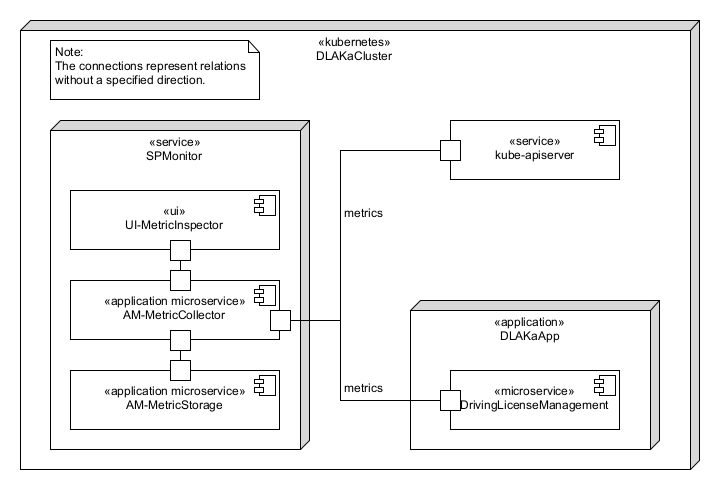
\includegraphics[width=\textwidth]{figures/abstract_sps_spmonitor.png}
	\caption{Abstract SystemPlusSoftware Architecture for SPMonitor}
	\label{fig:abstract_sps_spmonitor}
\end{figure}

% Based on the above analysis, an abstract SPS architecture was created for SPMonitor.
% The architecture can be seen in Figure \ref{fig:abstract_sps_spmonitor}.
% In this architecture, no concrete tools are considered. Instead, only abstract components
% and their interactions are visualized. These components and their interactions are based
% on the complete analysis of SPMonitor.
% SPMonitor will consist of two microservices and a user interface.
% The user interface provides the functionality of displaying the collected metrics
% in dashboards and graphs. The Data Source microservice is responsible for collecting
% the metrics from DLAKaApp. It also provides an interface for the user interface
% to access the stored values of the metrics. The Data Sink microservice handles the storage
% of the metric values and provides an interface to the Data Source for storing and accessing
% collected metric values.
% For the collection of the metrics, both the DLAKaApp and the DLAKaCluster need to provide
% and interface through which the Data Source microservice can collect their respective metrics.

\subsection{API Specification}

The abstract SPS architecture defined in Figure \ref{fig:abstract_sps_spmonitor} requires
the DLAKaApp to provide two interfaces through which SPMonitor can collect metrics.
The DLAKaCluster running in Kubernetes already provides the required interface 
through an HTTP endpoint at clusterURL/metrics. The application microservice DrivingLicenseManagement
will have to be adapted with a similar endpoint. It will also be hosted on the path /metrics
and export metrics in the same format as Kubernetes does. The actual format of the exported metrics
might have to change later if the data source that will be used requires a different format
but the endpoint will conceptually still be the same. The format used by Kubernetes is the Prometheus
metrics format. In this format, each metric is expressed as three lines of text. The first line
provides information about the meaning of the metric. The second line declares the type of metric.
In the case of NumDDL, this is a counter which is a positive integer that can never decrease.
The last line contains the name of the metric and its value. Optionally, the last line
can also contain a set of labels with assigned values. Labels are not used for the NumDDL metric.
The API specification of the metrics endpoint for DrivingLicenseManagement can be seen in Listing \ref{lis:api_spec_drivinglicensemanagement}
which is written using the OpenAPI standard.

\begin{lstlisting}[caption = {Partial API Specification of Application Microservice DrivingLicenseManagement}, label = {lis:api_spec_drivinglicensemanagement}, style = kit-cm, language=]
openapi: 3.0.0
info:
  title: Partial API of Application Microservice DrivingLicenseManagement
  version: 1.0.0
paths:
  /metrics:
    get:
      responses:
        200:
          description: Success
          content:
            text/plain:
              schema:
                type: string
              examples:
                has_value: 
                  summary: The metric has a value
                  value: |
                    # HELP num_ddl Number of issued digital driving licenses
                    # TYPE num_ddl counter
                    num_ddl 42
                no_value: 
                  summary: The metric has no value
                  value: |
                    # HELP num_ddl Number of issued digital driving licenses
                    # TYPE num_ddl counter
                    num_ddl 0
\end{lstlisting}

The API diagram of the application microservice DrivingLicenseManagement also needs to be adapted
to provide the functionality of exporting metrics on an HTTP endpoint. The API diagram
represents the logical connection between different endpoints in the style of Domain-Driven Design.
The changes to the diagram consist of two additional entities: The MetricsCollector and the Metric.
The Metric entity represents a single integer valued metric. Each metric has a name, a current value,
and an optional list of labels. The value of the metric can be updated or exported which constructs
a string in the format used by the API Specification in Listing \ref{lis:api_spec_drivinglicensemanagement}.
The MetricsCollector entity is a collection of Metric entities. While there is only one metric currently,
this design was chosen as it also extensions in the future. Through the MetricsCollector the value of
a metric can be updated by DrivingLicenseManagement. For the case of NumDDL, this update happens from
the createIssuance method which creates digital driving licenses.
The MetricsCollector also provides a method for exporting all metrics. This returns the combination
of each metric's representation as a string in the form of an HTTP response.
The exportAll method is the method that is responsible for handling the metrics endpoint. All other
added methods just provide the logic needed for exporting the metrics.
The adapted API diagram can be seen in Figure \ref{fig:api_diagram_drivinglicensemanagement}.

\begin{figure}[h]
	\centering
	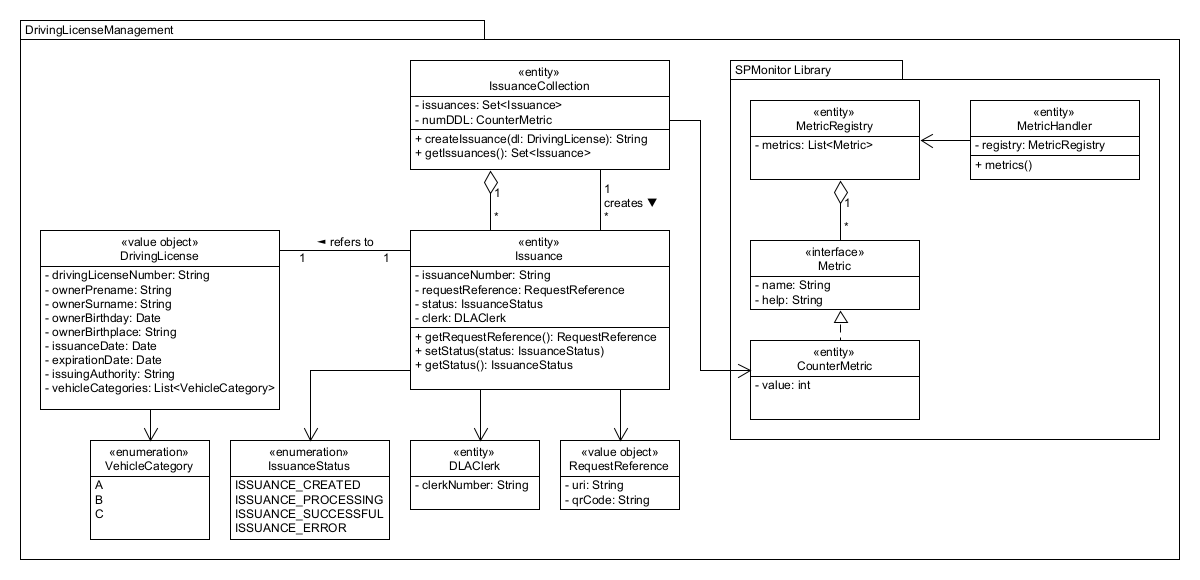
\includegraphics[width=\textwidth]{figures/api_diagram_drivinglicensemanagement.png}
	\caption{API Diagram DrivingLicenseManagement}
	\label{fig:api_diagram_drivinglicensemanagement}
\end{figure}

\todo{Describe and move}
\begin{figure}[h]
	\centering
	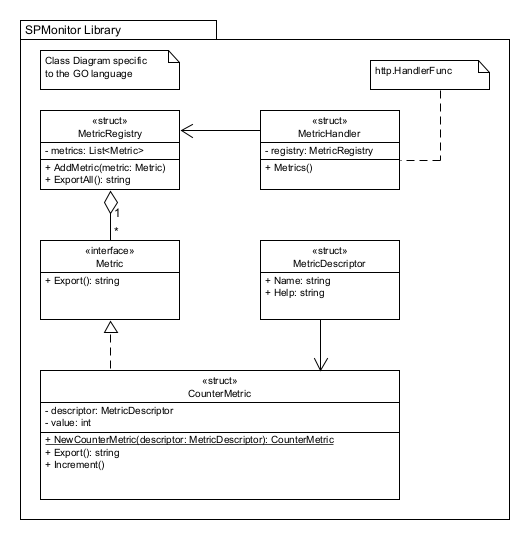
\includegraphics[width=\textwidth]{figures/class_diagram_spmonitor_library.png}
	\caption{Class Diagram SPMonitor Library}
	\label{fig:class_diagram_spmonitor_library}
\end{figure}

\subsection{Software Architecture}

\todo{Write}
\begin{figure}[h]
	\centering
	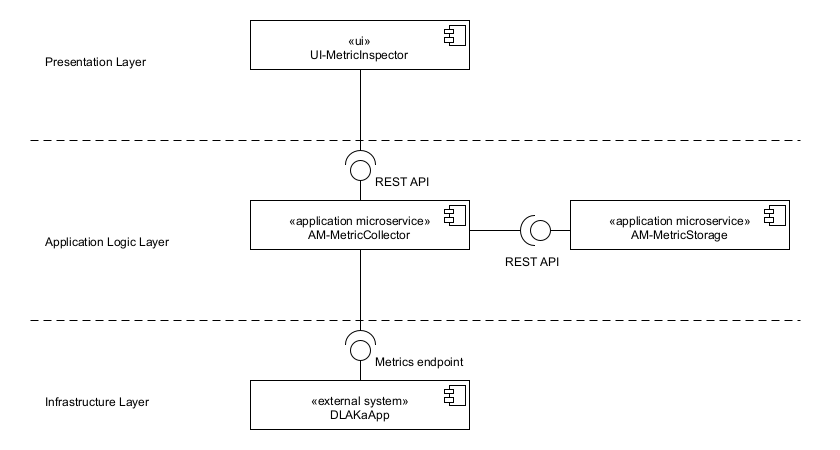
\includegraphics[width=\textwidth]{figures/software_architecture_sps.png}
	\caption{Software Architecture SPMonitor}
	\label{fig:sofware_architecture_spmonitor}
\end{figure}

\subsection{Tool Selection Based on Capabilities and Requirements}

\todo{Update to fit new layout}
As explained in Chapter \ref{cha:technical_foundation}, a monitoring system consists of three parts:
The Data Source, Data Sink and a tool for visualization.
The data source is the core of a monitoring system. It is responsible for collecting the monitoring data
and dictates the needs for the data sink as well as the possibilities for the visualization.
Because of its central role, the data source will be the first component of the monitoring system that will be chosen
and the rest of the monitoring system will be chosen to best fit with and support the data source.

In order for the chosen data source to best fit the needs of SPMonitor, it needs to fulfill some requirements
which stem from SPMonitor's use cases. The first requirement for the data source is that it should be built
to support the use cases of SPMonitor. Tools that are built for different purposes but could be used for SPMonitor's
use cases, will be less preferable than tools that are designed for SPMonitor's use cases.
Secondly, the data source should be free to use. This requirement mostly stems from the scope of this work
as a bachelor's thesis without any funding.
Additionally, the data source needs to be able to collect technical metrics as well as business metrics.
While technical metrics can be gathered from most cloud environments automatically, business metrics
require the instrumentation of the source code of the monitored services. Many data sources can in theory
instrument service but they often use additional tools like OpenTelemetry for this. Because SPMonitor aims
to be as slim as possible, to reduce complexity, data sources that can instrument services on their own without
the need for an additional tool, will be preferred over data sources that can not do that.
Lastly, the data source needs to support two different cloud environments: Kubernetes for the on-premise parts
of \Gls{DLAKaApp} and Microsoft Azure for the decentralized identity part of DLAKaApp.

These six requirements for the data source are listed in Table \ref{tab:data_source_requirements}.
Requirements R2 through R6 are hard requirements, meaning that a data source that does not fulfill them
will not be chosen. Requirement R1 is a soft requirement that is meant as an orientation and does directly
lead to the elimination of a data source.

\begin{table}[]
\centering
\begin{tabular}{c|l}
Key & Requirements \\
\hline
R1 & Purpose \\
R2 & Licensing \\
R3 & Technical metrics \\
R4 & Business metrics \\
R5 & Kubernetes \\
R6 & Microsoft Azure \\
\end{tabular}
\caption{Requirements for the Data Source}
\label{tab:data_source_requirements}
\end{table}

The data sources that will be compared according to the requirements in Table \ref{tab:data_source_requirements} stem
from the paper \enquote{A Survey on Observability of Distributed Edge {\&} Container-Based Microservices}
by Usman et al. \cite{UF+22}. The list from that survey was supplemented with one additional entry,
the TICK (Telegraf, InfluxDB, Chronograf, Kapacitor) stack. Any entries that do not support metrics or are purely research projects were eliminated.
Lastly, the entry for Kibana was changed to ELK for the ELK (ElasticSearch, LogStash, Kibana) stack.
The complete overview of all analyzed tools can be seen in Table \ref{tab:data_source_comparison}.

\begin{table}[]
\centering
\begin{tabular}{l|c|c|c|c|c|c}
Name & R1 & R2 & R3 & R4 & R5 & R6 \\
\hline
Apache SkyWalking		 & Performance & Free & \cmark & \cmark & \cmark & \xmark \\
Cilium					 & Networking & Free & \cmark & \xmark & \cmark & \cmark \\
Datadog					 & SaaS & Paid & \cmark & \cmark & \cmark & \cmark \\
Dynatrace				 & PaaS & Paid & \cmark & \xmark & \cmark & \cmark \\
ELK						 & Searching & Paid & \cmark & \xmark & \cmark & \cmark \\
Honeycomb				 & Debugging & Paid & \cmark & \cmark & \cmark & \cmark \\
Instana					 & Incidence Management & Paid & \cmark & \xmark & \cmark & \cmark \\
Monasca					 & MaaS & Free & \cmark & \xmark & \cmark & \xmark \\
New Relic				 & PaaS & Paid & \cmark & \cmark & \cmark & \cmark \\
\rowcolor{lightgray}
OpenTelemetry			 & Monitoring & Free & \cmark & \cmark & \cmark & \cmark \\
\rowcolor{lightgray}
Prometheus				 & Monitoring & Free/Paid & \cmark & \cmark & \cmark & \cmark \\
Scalyr					 & PaaS & Paid & \cmark & \xmark & \cmark & \xmark \\
SolarWinds				 & PaaS & Paid & \cmark & \xmark & \cmark & \cmark \\
Splunk					 & Resilience & Paid & \cmark & \cmark & \cmark & \cmark \\
Sumo Logic				 & Analytics & Paid & \cmark & \cmark & \cmark & \cmark \\
\rowcolor{lightgray}
TICK					 & Time Series Data & Free/Paid & \cmark & \cmark & \cmark & \cmark \\
\end{tabular}
\caption{Comparison of data sources}
\label{tab:data_source_comparison}
\end{table}

The three final candidates for use in SPMonitor can be seen highlighted in Table \ref{tab:data_source_comparison}.
They are OpenTelemetry, Prometheus, and the TICK stack.
OpenTelemetry is a standalone solution for the collection of metrics. 
It provides many client libraries to instrument service for business metrics and can integrate
with most data sinks and visualization tools.
Prometheus is commonly used in combination with the LGTM (Loki Grafana Tempo Mimir) stack.
Loki is a service for handling logs, Tempo is responsible for handling traces, Grafana is used for visualization and Mimir provides
long-term storage for Prometheus. Prometheus itself is responsible for the collection of metrics.
As this work only considers metrics, the full setup would use Grafana for visualization, Prometheus as the data source, and Mimir
as the data sink. As Mimir only provides Prometheus with an interface to a storage system and is itself not one, it can be paired with MinIO
a free-to-use object storage system.
The TICK stack consists of four different tools: Telegraf, InfluxDB, Chronograf, and Kapacitor.
Telegraf is responsible for collecting metrics from the monitored services. The collected metrics are then forwarded
to InfluxDB, the storage component of the stack, and Kapacitor which is responsible for data processing.
Chronograf provides the interface to visualize and analyze the collected metrics.

\begin{figure}[h]
	\centering
	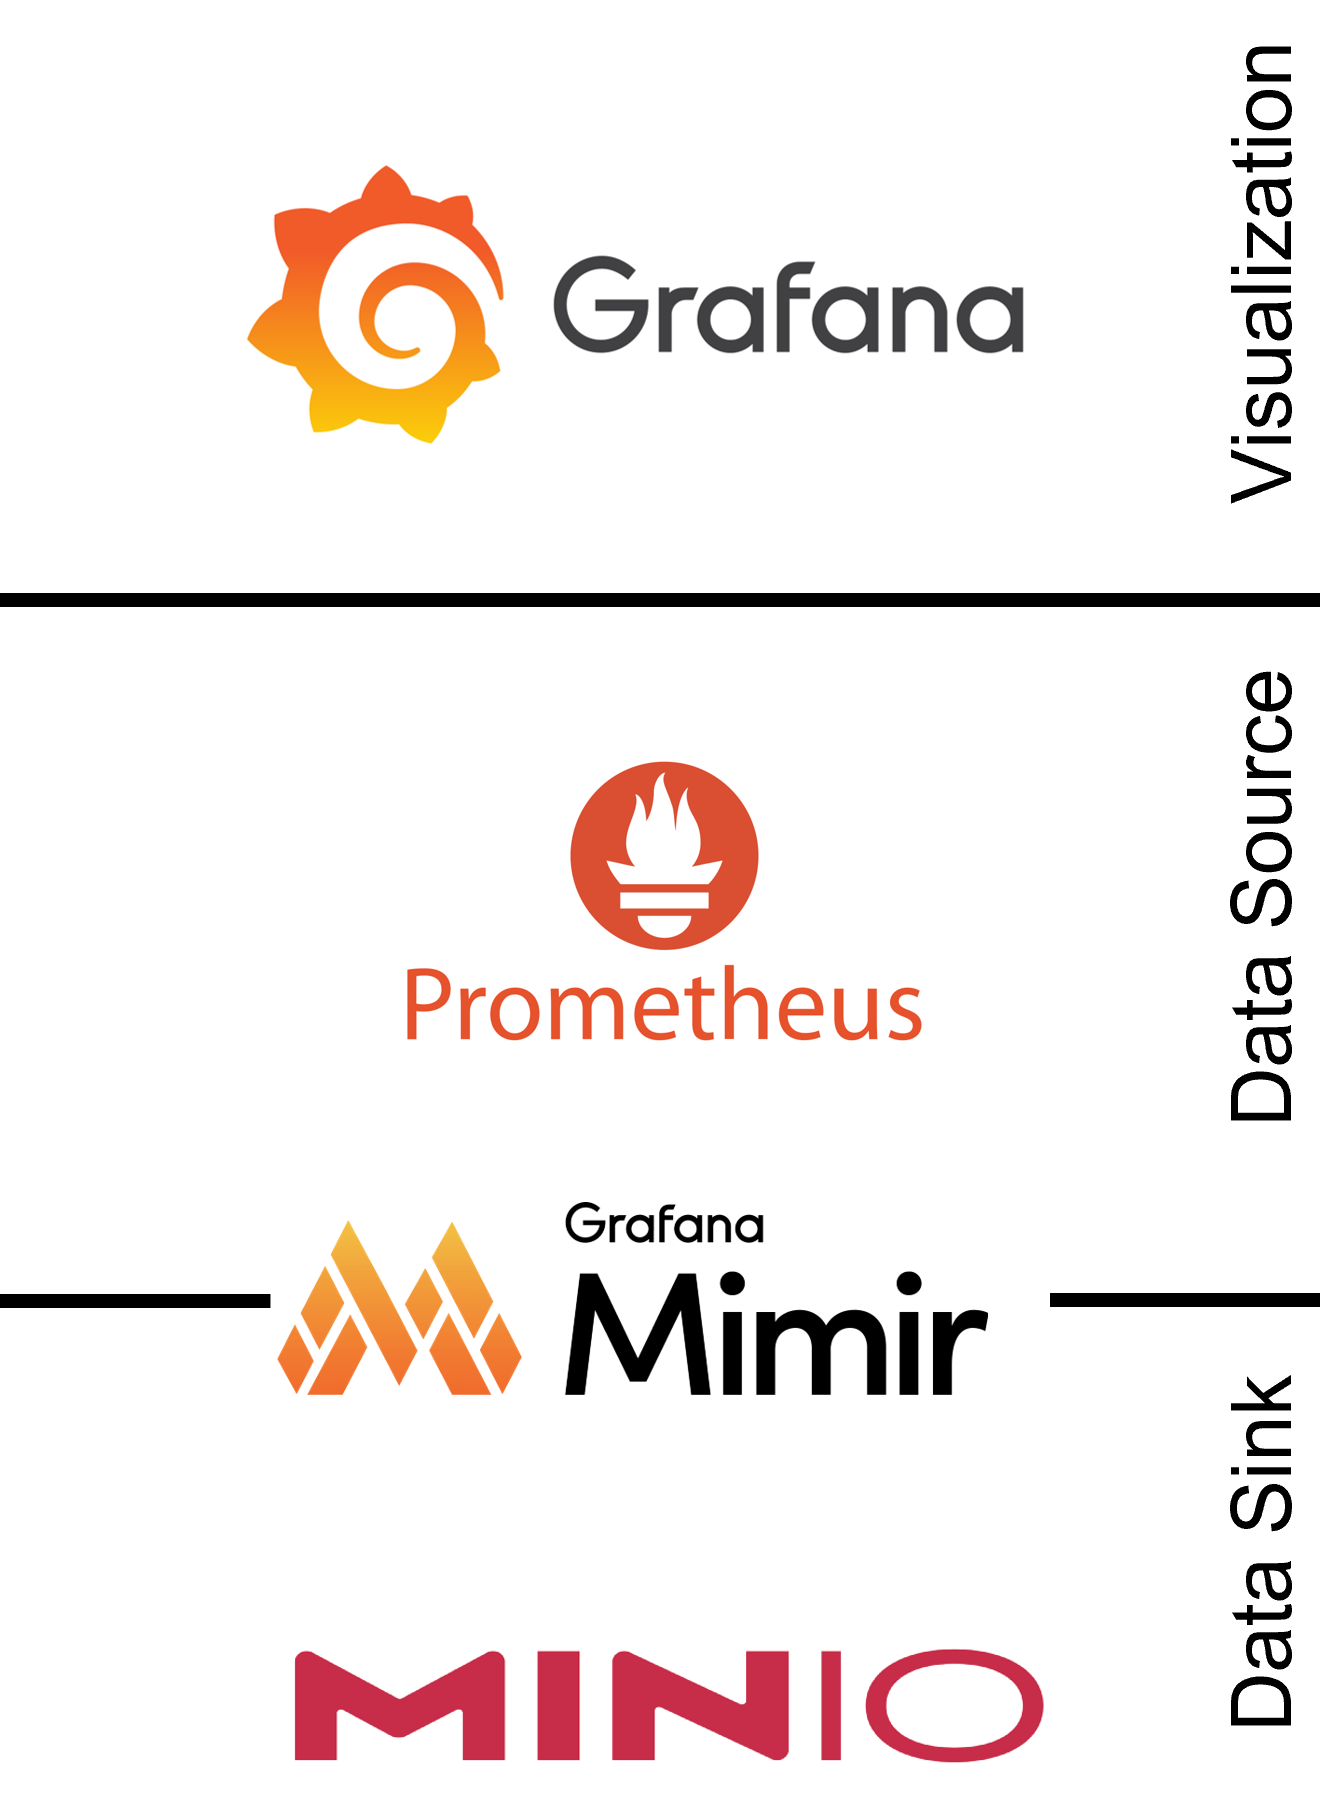
\includegraphics[width=0.4\textwidth]{figures/spmonitor_tech_stack.png}
	\caption{SPMonitor Technology Stack}
	\label{fig:spmonitor_tech_stack}
\end{figure}

From these three options, Prometheus together with Grafana, Mimir, and MinIO was chosen for SPMonitor.
Unlike OpenTelemetry, Prometheus provides easy integration with its data sink and visualization tool as
they were built to work together. OpenTelemetry on the other hand is a standalone solution meant to enhance
other tools which do not collect metrics themselves. The TICK stack provides the same integration benefit compared
to OpenTelemetry. The decision between Prometheus and the TICK stack is not as straightforward.
Both fulfill all requirements, offer extensibility options through plugins for different data sources
and pre-built visualizations, and they are both open-source projects which can be freely used.
One difference between them is that there exists a provider solution for managing Grafana with Crossplane.
This does not seem to exist for the TICK stack. Crossplane will be used to provision and operate the cloud
services of \Gls{DLAKaApp} and SPMonitor. Therefore Grafana and Prometheus are chosen for SPMonitor as they offer tools
for integrating them with Crossplane compared to the TICK stack. The final selection of tools can be seen in Figure \ref{fig:spmonitor_tech_stack}.

\subsection{SPS Architecture}

\todo{Write}
\begin{figure}[h]
	\centering
	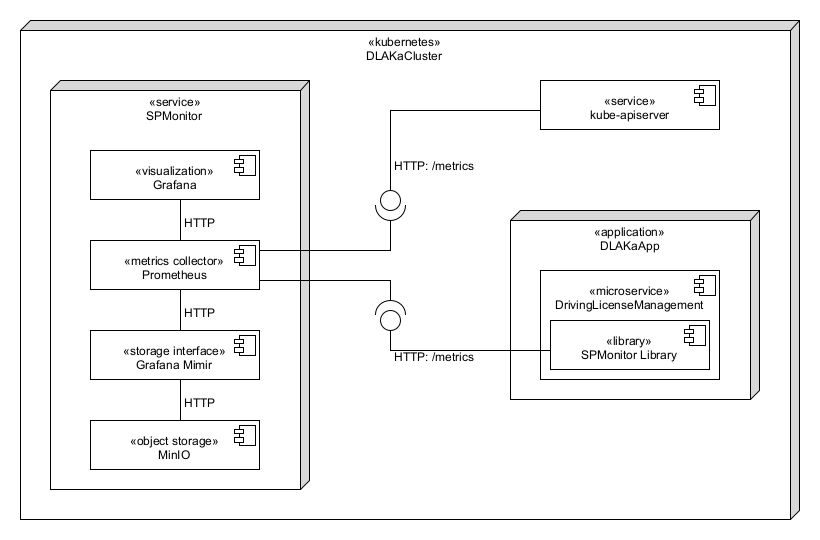
\includegraphics[width=\textwidth]{figures/sps_spmonitor.png}
	\caption{SystemPlusSoftware for SPMonitor}
	\label{fig:sps_spmonitor}
\end{figure}

\section{Implementation}

\todo{Do}

\section{Deployment}

\todo{Do}